\documentclass{jpc}
% Journal of Privacy and Confidentiality class (jpc.cls, github.com/journalprivacyconfidentiality/jpc-style).
% The layout macros \doisuffix and \jpcheading are added by the editorial team.
\usepackage{mathtools,booktabs,graphicx}
\usepackage{tikz}
\graphicspath{{./}{../}}
\usetikzlibrary{arrows.meta,positioning,fit,patterns,calc,shapes.geometric}
\usepackage{xr-hyper}
\externaldocument[S-]{jpc_supplement}
\makeatletter\g@addto@macro\UrlBreaks{\do\_\do\-}\makeatother
\newtheorem{theorem}[thm]{Theorem}
\newtheorem{proposition}[thm]{Proposition}
\newtheorem{assumption}[thm]{Assumption}
\theoremstyle{remark}
\newtheorem{remark}[thm]{Remark}
\newcommand{\Prob}{\mathbb P}
\newcommand{\E}{\mathbb E}
\newcommand{\F}{\mathcal F}
\keywords{disclosure risk, sequential testing, test supermartingale, online multiple testing, composition attack, official statistics}
\begin{document}
\title[Adaptive certification of disclosure risk]{Adaptive certification of attack-conditional disclosure risk across release programmes}
\author{Ronald Rethabile Malamule Mahomane}
\address{Department of Computing, Mathematical and Statistical Sciences, University of Namibia, Windhoek; School of Pathology, Faculty of Health Sciences, University of the Witwatersrand, Johannesburg; Basis Energy, Victoria, Australia}
\email{ron@basisenergygroup.com}
\begin{abstract}
An agency that publishes a series of releases from one register must decide which releases are safe against a list of attacks that grows as audits are read, and it must be able to show that the audit itself was not gamed. We treat each pair of a candidate release and a declared attack as a risk coordinate, certified when a betting test supermartingale for the hypothesis that its success probability is at least its tolerance crosses a threshold fixed at registration. Under a stated condition on how attack targets are sampled, the chance of ever certifying a coordinate at or above its tolerance is at most the error budget, even when coordinates are added after outcomes are seen and audits stop at will. The error control is online alpha-spending; what we add is specific to disclosure audits: a bound on expected audit length set by the gap between risk and tolerance, release chains that choose a setting from an ordered grid and test every declared attack at the full level, and a threat model for the audit process with measured attacks on it. On a synthetic credit register with six monthly vintages in which loans enter and leave, per-release review passes the file with no suppression. An adversary who pools the vintages and knows when the target's loan was live needs a cell-count floor of 75, and one who also holds an exposure reading per vintage needs 150, which keeps a fifth of the loans and under four per cent of the exposure; an insider who knows exposure to within one per cent defeats every floor tested. A release chain over the three declared attacks chose 150 in 19 of 20 attack streams and never chose an unsafe floor. An operator who can choose among a hundred seeds certifies an attack at the tolerance in 98 per cent of runs, and one who bets after seeing outcomes certifies an unsafe attack in every run; committed randomness and committed bets close both routes if the registry itself is trusted.
\end{abstract}
\maketitle

\renewcommand{\thefootnote}{\fnsymbol{footnote}}
\footnotetext[1]{Overlap with earlier work. Table~\ref{tab:carried} and the four-release and public-file figures in Section~\ref{sec:carried} reproduce results first reported in \cite{mahomane2026}, an author manuscript whose earlier version was presented at the Banco de Portugal and IFC Workshop on Data Security and Privacy, Lisbon, September 2026; Figure~\ref{fig:pool} is adapted from it. Theorem~\ref{thm:gate}, Propositions~\ref{prop:cost} to~\ref{prop:release}, the toy audit (Table~\ref{tab:new-audit}), the credit-register audit (Table~\ref{tab:chain-audit}), the factor-by-factor floors and the audit-process measurements (Table~\ref{tab:audit-process}) are new. The credit register itself has been revised since \cite{mahomane2026}: loans now leave for good and new loans enter each month, and the pooled attack uses absence as well as presence in the target's history.}
\renewcommand{\thefootnote}{\arabic{footnote}}

\section{Introduction}\label{sec:intro}
Statistical agencies and central banks rarely publish one file. They publish a monthly or quarterly series from the same register, such as the loan-level credit registers that researchers use to separate the supply of credit from its demand \cite{khwaja2008}, and each new release overlaps the previous ones in the units it covers. Disclosure review, by contrast, is usually done one release at a time: a release passes if its own risk measure falls below a limit. Two facts make this unsafe. First, an adversary who holds several releases can combine them, so that the risk of the programme is not a function of the risks of its parts \cite{sweeney2002,ganta2008}. Second, the list of attacks worth testing is not fixed in advance. Disclosure officers read the results of one audit and then propose another attack, a new subgroup or a pooled version of an attack already run. A procedure that controls error for a family fixed in advance does not cover a family that grows in response to its own results.

This paper sets out a release gate for that situation. Each pair of a candidate release and a declared attack is a \emph{risk coordinate}: a success event, a target law and a tolerance chosen by the agency. The success probability of a coordinate is estimated by running the attack on freshly drawn targets. A coordinate is certified when a betting test supermartingale for the null hypothesis ``risk at least tolerance'' crosses a threshold fixed when the coordinate is registered, and a release is eligible only when every coordinate the policy declares for it is certified.

The error control is standard. Each coordinate receives a share of the error budget at registration, as in online alpha-spending \cite{foster2008,tian2021}, and each share is spent through Ville's inequality on a test supermartingale \cite{ville1939,shafer2011,ramdas2023}. What we add is the part that is specific to disclosure audits:
\begin{enumerate}
\item a definition of a risk coordinate, with a formal threat model for pooled attacks on several vintages that separates what the adversary holds (releases, readings, and the target's history) and shows when pooled attacks need coordinates of their own (Section~\ref{sec:setting});
\item a condition on how attack targets are sampled (Assumption~\ref{ass:law}) under which the gate is valid, and examples of audit designs that break it;
\item three results on the cost of the gate: the zero-success cost, a bound on the expected audit length when the risk lies below the tolerance, and the allocation of the budget that minimises expected cost (Propositions~\ref{prop:cost}, \ref{prop:length} and~\ref{prop:weights});
\item chained registration and release chains: coordinates registered one after another, each only after its predecessor certifies, share one allocation, and a release setting with several declared attacks can test each at the full level (Propositions~\ref{prop:chain} and~\ref{prop:release}), which is how a floor is chosen from a grid without a multiplicity penalty;
\item a run of the gate on a synthetic credit register that chooses a cell-count floor against three declared adversaries, compared draw for draw with five other designs and checked for validity on Bernoulli streams at the estimated risks (Section~\ref{sec:credit});
\item a threat model for the audit process itself, with an operator who can grind seeds, run shadow audits or bet after seeing outcomes, measured attacks on it, and implemented controls (Section~\ref{sec:security}).
\end{enumerate}

Section~\ref{sec:related} reviews related work. Section~\ref{sec:setting} states the threat model and the estimands. Section~\ref{sec:gate} gives the gate and its theory. Section~\ref{sec:experiments} reports the experiments, Section~\ref{sec:security} sets out the security properties, Section~\ref{sec:discussion} the limits, and Section~\ref{sec:conclusion} concludes. The supplement holds proof details, the proposal model, and reproduction commands.

\section{Related work}\label{sec:related}
\paragraph{Online error control and test supermartingales.} Wald's sequential probability ratio test \cite{wald1945} stops as soon as the evidence is strong enough, and confidence sequences \cite{darling1967,robbins1970,lai1976} give intervals that hold at every sample size at once. Monitoring an experiment with fixed-sample tests and stopping on a good result inflates the error rate; always-valid $p$-values correct this for online experiments \cite{johari2022}. Fixed-sample methods for many hypotheses use the Bonferroni bound \cite{dunn1961} or control the false discovery rate \cite{benjamini1995}, and inference after a model has been chosen from the data needs its own correction \cite{berk2013}. Alpha-investing \cite{foster2008} controls a false discovery measure, and online control of the familywise error rate \cite{tian2021} controls the familywise error, over a sequence of hypotheses whose length and order need not be known in advance; the simplest online rule, online Bonferroni, gives the $i$th hypothesis a level $\alpha w_i$ with $\sum_iw_i\le1$. Generalized alpha-investing \cite{aharoni2014} and online rules for the false discovery rate \cite{javanmard2018} extend this to weaker error measures. Test supermartingales and e-values \cite{shafer2011,vovk2021,ramdas2023} turn a sequence of observations into evidence that remains valid under optional stopping, through Ville's inequality \cite{ville1939}; game-theoretic probability supplies their foundations \cite{shafer2019}, safe tests build them for composite hypotheses \cite{grunwald2024}, and e-values can also control the false discovery rate \cite{wang2022}. Nonnegative supermartingales give time-uniform concentration bounds \cite{howard2020}, and betting constructions give confidence sequences for bounded means \cite{howard2021,waudby2024}. Theorem~\ref{thm:gate} is online Bonferroni applied to such betting processes. Risk-controlling prediction sets \cite{bates2021}, their active and anytime-valid version \cite{xu2024} and adaptive auditing of AI systems with simultaneous e-processes \cite{zhou2026} combine predictors with sequential evidence in the same way. Risk-limiting audits of elections are the closest use of the same tool: they sample ballots, bet on each draw with a predictable alternative, often a shrunk running mean, and certify an outcome when a test supermartingale crosses a threshold \cite{stark2008,waudby2021,stark2023}. The bet rule in Section~\ref{sec:credit} is of that kind. Our outcome differs: a disclosure attack on a named target law, with coordinates that include pooled vintages, and a search over release settings rather than one reported outcome. Choosing among ordered settings without splitting the error budget is fixed-sequence testing \cite{maurer1995,hsu1999}, and graphical and gatekeeping procedures generalise it \cite{dmitrienko2007,bretz2009}; Propositions~\ref{prop:chain} and~\ref{prop:release} carry the fixed-sequence and intersection-union arguments \cite{berger1982} over to adaptively registered e-processes.

\paragraph{Composition and intersection attacks.} That releases which are each safe under a syntactic rule can be joined to re-identify people is well known. Sweeney described complementary and temporal attacks on $k$-anonymous releases \cite{sweeney2002}; sequential releases were studied by \cite{wang2006}; Ganta, Kasiviswanathan and Smith showed that independently protected releases can be composed into an attack \cite{ganta2008}; and many accurate answers permit reconstruction \cite{dinur2003}. Proposition~\ref{prop:pool} below is an example of this kind. We use it only to fix the estimand the gate must certify.

\paragraph{Privacy auditing.} Membership inference attacks test whether a record was in a model's training set \cite{shokri2017}, and their success is best judged by the true-positive rate at a low false-positive rate \cite{carlini2022}. Audits of differentially private training estimate a lower bound on leakage from the success of an attack, using exact binomial intervals \cite{jagielski2020,nasr2021,steinke2023}. The gate uses the same primitive in the other direction: it upper-bounds the success of one declared attack in order to certify, and so it speaks only to that attack. Tight audits of private training \cite{nasr2023} and black-box testers that search for violations of a claimed $\varepsilon$ \cite{ding2018,bichsel2021} are the same idea at the level of a mechanism, and attacks on synthetic data \cite{stadler2022} show how far syntactic protection can fall short. Auditing by betting has also been used for fairness \cite{chugg2023}. With its null reversed, the gate is a sequential lower-bound auditor for a claimed privacy level. The hypothesis-testing view of differential privacy \cite{wasserman2010,kairouz2017} bounds the success of every attack on an $(\varepsilon,\delta)$-private release by $e^\varepsilon\kappa+\delta$, where $\kappa$ is the attack's success when the target's record is replaced, so for such releases a tolerance $\tau$ is met by all attacks at once when $e^\varepsilon\kappa+\delta\le\tau$. That analytic bound is stronger than any certificate the gate can give, which covers declared attacks only; the gate is for releases, such as suppressed microdata, that have no privacy parameter.

\paragraph{Disclosure risk measures.} Statistical disclosure control defines risk through an intruder's scenario, knowledge and matching rule \cite{duncan1989,hundepool2012}, and estimates identification risk from models of the sample and population \cite{skinner2008}, from the probability that an intruder's match is correct given the released data \cite{reiter2005}, or under misclassification of released values \cite{shlomo2010}. A systematic review of re-identification attacks on health data records the data on which such attacks have succeeded \cite{elemam2011}, and $k$-anonymity algorithms have been adapted to health data \cite{elemam2008}. Few attributes make most people unique: four spatio-temporal points single out most people in a mobility dataset \cite{demontjoye2013}, a generative model can estimate the chance that a match in an incomplete sample is correct \cite{rocher2019}, and sparse records can be linked to public profiles with little auxiliary knowledge \cite{narayanan2008}. Differential privacy \cite{dwork2014} bounds how far any adversary's odds about one record can move relative to that record's absence \cite{kasiviswanathan2014}; it does not report the success probability of a named linkage attack. Its guarantees depend on assumptions about how records are correlated \cite{kifer2011}, which the Pufferfish framework makes explicit through declared secrets and data laws \cite{kifer2014}; Gaussian differential privacy states the guarantee as a trade-off between the errors of a test for one record \cite{dong2022}. The U.S. Census Bureau adopted differential privacy for its 2020 products \cite{abowd2018}, and legal notions such as the singling out named in the GDPR have been given formal statements \cite{cohen2020}. The risk coordinate here is an intruder scenario in this tradition, made precise enough to be audited by sampling.

\section{Setting, threat model and estimands}\label{sec:setting}
\subsection{Releases, adversary and success event}
Let $U$ be a finite population of units and $\theta$ a candidate release mechanism, such as a cell-count floor. A programme publishes releases $D_{\theta,1},\ldots,D_{\theta,V}$, one per vintage, each covering the units present at that vintage. A \emph{scenario} $a$ names an attacker, a harm, a subgroup and the set of vintages the attacker holds; a scenario that holds more than one vintage is a pooled attack. The pair $i=(\theta,a)$ is a risk coordinate. We state the threat model for the identification harm used in the experiments; other harms need their own success events but enter the gate in the same way.

\begin{assumption}[Threat model]\label{ass:threat}
(i) \emph{Release format.} Release $v$ publishes, for every unit it contains, a pseudonym that is the same in every vintage, the unit's published key $K_v(u)$ and any other published attributes. (ii) \emph{Knowledge.} The adversary knows the target's full vector of quasi-identifiers, from which it can form the published key of every release, and the auxiliary readings the scenario declares; it knows that the target is present in the first release it holds; it holds the releases in the scenario's vintage set; and, when the scenario says so, it knows in which of those vintages the target is present (its \emph{history}). (iii) \emph{Decision.} The adversary names one pseudonym, $d_a(Z_t,D_\theta)$, by a rule declared with the scenario, where $Z_t$ is its information about target $t$. (iv) \emph{Success.} The attack succeeds on $t$ if the named pseudonym is the target's.
\end{assumption}

Write $S_i(t)$ for the success event of coordinate $i$ on target $t$. The \emph{identification probability} of coordinate $i$ is
\begin{equation}\label{eq:risk}
r_i=\Prob_{t\sim T_i}\{S_i(t)\},
\end{equation}
where $T_i$ is the target law and the probability also covers the noise in the adversary's readings and any random tie-breaking. The agency sets a tolerance $\tau_i\in(0,1)$. Neither $r_i$ nor $\tau_i$ is a differential privacy parameter. The experiments use $\tau=0.12$ for an average over prosecutor targets; guidance for public release of clinical data uses 0.09 for average risk \cite{ema2016}, and we report floors at 0.05, 0.09 and 0.20 as well (Table~\ref{tab:tolerance-floors}). Under European statistical law a tolerance is the institution's written reading of when identification is reasonably likely \cite{ec2533}, and it should be owned by the body that answers for that reading. The target law matters: a prosecutor scenario draws targets known to be in the release, a journalist scenario draws from the population, and the same attack has different $r_i$ under the two laws \cite{duncan1989,hundepool2012}. In the classical special case where the adversary observes the target's exact key, the $f$ released units sharing that key are exchangeable given the adversary's information and the adversary picks one at random, the conditional success probability is $1/f$, and $k$-anonymity gives $r_i\le1/k$. Informative auxiliary readings break the exchangeability, and the success probability can then exceed $1/f$.

The history in (ii) is a separate piece of knowledge and it matters. A borrower knows when its own loan was drawn and repaid, and so does its lender; charges and security interests are often registered publicly; a journalist or a researcher working from the releases alone usually does not know them. On the register of Section~\ref{sec:credit}, where a loan's published key and exposure do not change between vintages and whether a loan is live is drawn independently of both, the other vintages carry no information about which candidate is the target unless the adversary knows the target's history. That holds by construction of the generator and would not hold on a register whose outstanding amounts change from month to month. The history cuts both ways: an adversary who knows it can exclude every candidate whose pattern of appearances differs from the target's, including candidates that appear in a vintage where the target does not. Most parties who know a loan's history, such as the borrower and its lenders, also know its exposure exactly; we treat that insider as a separate adversary.

\subsection{Pooled attacks need their own coordinates}
Let $S_v$ be success from vintage $v$ alone. The chance that some single vintage succeeds obeys
\begin{equation}\label{eq:union}
\max_v\Prob(S_v)\le\Prob\Bigl(\bigcup_vS_v\Bigr)\le\min\Bigl(1,\sum_v\Prob(S_v)\Bigr).
\end{equation}
An adversary who holds all vintages can intersect candidate sets through the persistent pseudonym, and its success event $S_{\rm pool}$ is not $\bigcup_vS_v$.

\begin{proposition}[Marginal risks do not bound pooled risk]\label{prop:pool}
Under Assumption~\ref{ass:threat}, for every $\nu>0$ and $V\ge2$ there is a population and $V$ releases, each $s$-anonymous with identification probability at most $\nu$ under uniform target sampling and uniform tie-breaking, such that the pooled attack identifies every target.
\end{proposition}
\begin{proof}
Take an integer $s\ge1/\nu$ and let the population contain one unit for each $x\in\{1,\ldots,s\}^V$, all present in every vintage. Let release $v$ publish each unit's pseudonym and the key $K_v(x)=(x_1,\ldots,x_{v-1},x_{v+1},\ldots,x_V)$. Each key class of release $v$ has $s$ units, so the release is $s$-anonymous and its identification probability is $1/s\le\nu$. The candidate set from release $v$ is the set of pseudonyms whose units agree with $t$ in every coordinate except possibly the $v$th. For each coordinate $j$ there is a release $v\ne j$, since $V\ge2$, whose candidate set forces $x_j=t_j$; so the intersection of the $V$ candidate sets is the target's pseudonym alone, and pooled success is one.
\end{proof}

\begin{figure}[t]\centering
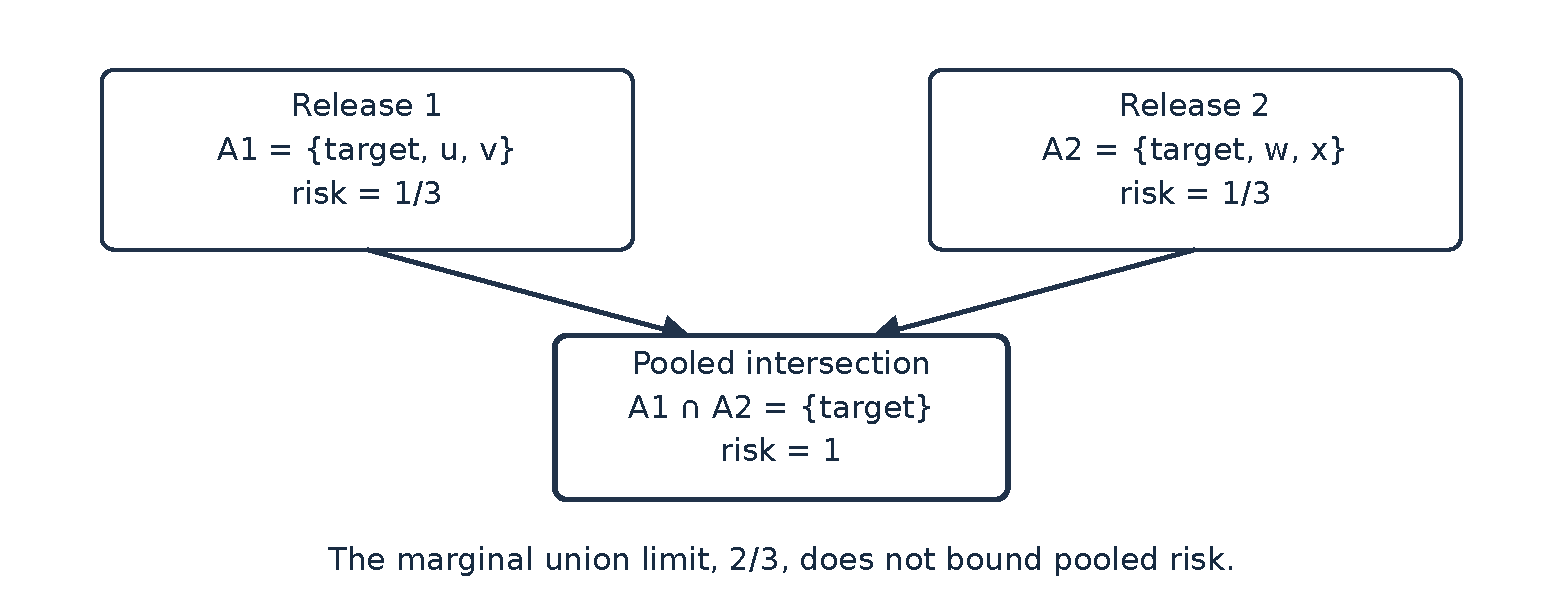
\includegraphics[width=.95\linewidth]{../diagrams/pooling.pdf}
\caption{Two releases that each leave three candidates for the target. Their intersection through the persistent pseudonym leaves one, so the pooled risk is one while the bound~\eqref{eq:union} on single-release success is two thirds.}\label{fig:pool}
\end{figure}

Figure~\ref{fig:pool} shows the smallest case. Each release leaves the target among three candidates, so each alone names the target with probability one third, and the sum of the two single-release risks is two thirds. The two candidate sets share only the target's pseudonym, so the pooled attack names it with certainty. Neither the phenomenon nor the construction is new: complementary and sequential releases that are each $k$-anonymous can be joined to re-identify people \cite{sweeney2002,wang2006,xiao2007}, independently protected releases can be composed into an attack \cite{ganta2008}, and many accurate answers permit reconstruction \cite{dinur2003}. We state it to fix the estimand: a pooled attack that the policy wishes to bound must be registered as a coordinate of its own, because no function of the per-release risks bounds it.

With a persistent pseudonym, releases that publish different projections of the quasi-identifiers can be joined into one table keyed on their union, so Proposition~\ref{prop:pool} says that the programme is one finer release. That suggests rotating the pseudonym between vintages as a cheaper remedy than any audit. It does not help when a published value that identifies the unit stays the same: on the register of Section~\ref{sec:credit}, with exposure published exactly, the pair of key and exposure is unique for every released loan, so each loan can be relinked across vintages from published fields alone. Publishing exposure to one significant figure leaves 10 per cent of loans unique in the first release, so rotation would then remove most of that route; small fresh noise in each vintage would not, since probabilistic record linkage copes with it. Rotation controls linkability; it is not pseudonymisation in the legal sense, which concerns keeping the key that re-identifies units apart \cite{gdpr2016}, and pseudonyms should be keyed so that they cannot be reversed by trying every identifier.

\subsection{From a risk vector to a decision}\label{sec:decision}
A policy declares, for each candidate release, a finite set of coordinates with tolerances $\tau_i$. Let $\alpha\in(0,1)$ be the familywise error level the agency accepts. If $B$ attacks on fresh targets produce $Y$ successes, the exact one-sided Clopper--Pearson upper bound at level $\lambda$ is
\begin{equation}\label{eq:cp}
\overline{R}(Y,B;\lambda)=\begin{cases}1,&Y=B,\\F^{-1}_{\mathrm{Beta}(Y+1,B-Y)}(1-\lambda),&Y<B,\end{cases}
\end{equation}
with $\overline{R}=1-\lambda^{1/B}$ when $Y=0$. For a family of $M$ coordinates fixed before any outcome is seen, $\lambda=\alpha/M$ and a union bound \cite{dunn1961} give simultaneous coverage without assuming the audits are independent. The \emph{audited margin} of coordinate $i$ is then $z_i=1-\overline{R}_i/\tau_i$, and a release is eligible within the declared family when $\min_iz_i\ge0$. That argument fails once the agency reads the audit, adds a coordinate and audits again at the same nominal level: the family is no longer fixed, a problem that also arises for inference after a model is chosen from the data \cite{berk2013}. The gate of Section~\ref{sec:gate} covers that case. It yields a binary decision, not an upper bound; to report an audited margin after adaptive registration, $\overline{R}_i$ must come from a time-uniform confidence sequence \cite{howard2021,waudby2024} with a registered share of the error budget.


\section{The registered gate and its theory}\label{sec:gate}
\subsection{Registration, filtration and the sampling condition}
Audits and registrations happen in global steps $g=0,1,2,\ldots$; at each step one thing is recorded (a development result, a proposed scenario, a registration or one audit outcome). Let $\F_g$ be the $\sigma$-field generated by everything recorded up to step $g$. Coordinate $i$ is registered at a stopping time $\sigma_i$ (with $\sigma_i=\infty$ if it never is), at which its identity $(\theta_i,a_i)$, its tolerance $\tau_i$, its attack protocol and its error allocation $w_i\ge0$ are fixed. Its $b$th audit outcome $X_{i,b}\in\{0,1\}$ is recorded at a stopping time $\gamma_{i,b}>\sigma_i$, and $\F_{\gamma_{i,b}-}=\F_{\gamma_{i,b}-1}$ is the $\sigma$-field just before that draw. Allocations must satisfy $\sum_iw_i\le1$ on every path, including coordinates that are withdrawn. Proposals from a model, a language model or a reviewer may lead to a registration; they are not audit outcomes.

\begin{assumption}[Conditional attack validity]\label{ass:law}
For each registered coordinate $i$, on the event $H_i=\{r_i\ge\tau_i\}$ and for every $b$ with $\gamma_{i,b}<\infty$,
\begin{equation}\label{eq:conditional}
\E[X_{i,b}\mid\F_{\gamma_{i,b}-}]\ge\tau_i .
\end{equation}
\end{assumption}
The condition holds when each draw uses a fresh target drawn from the registered target law, with fresh auxiliary noise, independently of everything recorded so far. It is stronger than a statement about the marginal mean. Repeating an attack on a target that has already failed, sharing a hidden target feature across interleaved audit streams, or changing the attacker's information after seeing outcomes can each break it (Supplement, Section~\ref{S-sec:s-filtration}).

\subsection{The gate}
Before each draw choose a predictable alternative $q_{i,b}\in[0,\tau_i)$, that is, one that is $\F_{\gamma_{i,b}-}$-measurable. Set $E_{i,0}=1$ and
\begin{equation}\label{eq:bet}
E_{i,b}=E_{i,b-1}\Bigl(\frac{q_{i,b}}{\tau_i}\Bigr)^{X_{i,b}}\Bigl(\frac{1-q_{i,b}}{1-\tau_i}\Bigr)^{1-X_{i,b}} .
\end{equation}
The factor is the likelihood ratio of a Bernoulli$(q_{i,b})$ outcome to a Bernoulli$(\tau_i)$ outcome, as in Wald's sequential probability ratio test \cite{wald1945}, with an alternative that may change from draw to draw. A success multiplies the evidence by $q_{i,b}/\tau_i<1$ and a failure by $(1-q_{i,b})/(1-\tau_i)>1$. Coordinate $i$ is certified at the first $b$ with $E_{i,b}\ge(\alpha w_i)^{-1}$, and it accepts no later outcomes; a coordinate with $w_i=0$ is never certified. A candidate release is eligible only if every coordinate the policy declares for it, pooled attacks included, has been registered and certified. A coordinate that has not been audited is not treated as having zero risk.

\begin{theorem}[Familywise control under adaptive registration]\label{thm:gate}
Suppose that (a) $(\theta_i,a_i)$, $\tau_i$ and $w_i$ are $\F_{\sigma_i}$-measurable, with $w_i=0$ on $\{\sigma_i=\infty\}$; (b) the index of the coordinate audited at each step is $\F_{g-1}$-measurable; (c) each $q_{i,b}\in[0,\tau_i)$ is $\F_{\gamma_{i,b}-}$-measurable; (d) $\sum_iw_i\le1$ on every path; and (e) Assumption~\ref{ass:law} holds. Then, for any countable sequence of registrations and any rule for stopping or continuing audits based on $(\F_g)$,
\begin{equation}\label{eq:family}
\Prob\bigl\{\exists i,b:\ r_i\ge\tau_i\ \text{and}\ E_{i,b}\ge(\alpha w_i)^{-1}\bigr\}\le\alpha .
\end{equation}
Hence, with probability at least $1-\alpha$, every eligible release meets every tolerance declared for it, whichever eligible release is chosen.
\end{theorem}

\begin{proof}
Fix $i$ and write $E_i(g)=E_{i,N_i(g)}$, where $N_i(g)$ counts the outcomes of coordinate $i$ recorded by step $g$; the process is constant between its own draws. For $p\ge\tau$ and $q<\tau$,
\[
p\frac q\tau+(1-p)\frac{1-q}{1-\tau}=1+\frac{(p-\tau)(q-\tau)}{\tau(1-\tau)}\le1 .
\]
By (b), (c) and~\eqref{eq:conditional}, on $H_i$ the conditional expectation of each factor given $\F_{\gamma_{i,b}-}$ is at most one, so $(E_i(g))_{g\ge\sigma_i}$ is a nonnegative supermartingale with respect to $(\F_g)$ that starts at one. Because $r_i$ is a function of the registered scenario $(\theta_i,a_i)$ and $\tau_i$ is fixed at registration, (a) makes $\mathbf 1_{H_i}$ and $w_i$ $\F_{\sigma_i}$-measurable. Ville's inequality \cite{ville1939}, applied conditionally on $\F_{\sigma_i}$, gives $\Prob(A_i\mid\F_{\sigma_i})\mathbf 1_{H_i}\le\alpha w_i\mathbf 1_{H_i}$, where $A_i$ is the event that coordinate $i$ crosses its threshold. Taking expectations, $\Prob(A_i\cap H_i)\le\alpha\E[w_i]$. A union bound over $i$, monotone convergence and (d) give~\eqref{eq:family}. On the complement of the event in~\eqref{eq:family}, no coordinate with $r_i\ge\tau_i$ is certified, so every eligible release meets every declared tolerance.
\end{proof}

\begin{remark}
Theorem~\ref{thm:gate} is the online Bonferroni rule \cite{tian2021} applied to betting test supermartingales \cite{shafer2011,waudby2024}. It is stated here to make conditions (a)--(e) explicit for attack audits. Condition (e) is where audit design enters: it concerns target sampling, not the accuracy of any model. The e-process $E_{i,b}$ is evidence for a binary decision. Neither $E_{i,b}$ nor $1/E_{i,b}$ is a risk estimate or an upper bound on $r_i$.
\end{remark}

\subsection{Audit cost and allocation}
\begin{proposition}[Zero-success cost]\label{prop:cost}
For a registered coordinate with $q_{i,b}=0$ for all $b$, after $B$ failures $E_{i,B}=(1-\tau_i)^{-B}$, so the coordinate can first be certified after
\begin{equation}\label{eq:budget}
B_{0,i}=\Bigl\lceil\frac{\log(1/(\alpha w_i))}{-\log(1-\tau_i)}\Bigr\rceil
\end{equation}
failures. A single success sets this process to zero, after which it cannot cross.
\end{proposition}
The proof is immediate from~\eqref{eq:bet}. With equal weights $w_i=1/M$, $B_{0,i}$ equals the zero-success sample size of a fixed family of $M$ one-sided Clopper--Pearson tests \cite{clopper1934}: for $M=8$, $\alpha=.05$ and $\tau=.12$ it is 40 attacks. The zero-alternative test is anytime-valid, so monitoring it throughout costs nothing in this case; the cost of anytime validity appears only when the bet must leave room for successes, as it must when the true risk is near the tolerance. A programme with no fixed end can set $w_i=6/(\pi^2i^2)$; the log-threshold of the $i$th coordinate then grows as $2\log i+O(1)$. A fixed family can be combined with a reserve for later coordinates (Supplement, Section~\ref{S-sec:s-allocation}).

The zero-alternative bet is the right one only if the audit expects no successes. When the risk lies below the tolerance but not far below it, as for the pooled coordinates in Section~\ref{sec:credit}, the cost is set by the gap between them.

\begin{proposition}[Expected audit length]\label{prop:length}
Let the outcomes of coordinate $i$ be independent Bernoulli$(p)$ with $p<\tau_i$, let the bet be fixed at $q\in(0,\tau_i)$, and write $A_i=\log(1/(\alpha w_i))$, $u=\log\{(1-q)/(1-\tau_i)\}$ and
\begin{equation}\label{eq:drift}
\mu(p,q)=p\log\frac q{\tau_i}+(1-p)\log\frac{1-q}{1-\tau_i}.
\end{equation}
If $\mu(p,q)>0$, the number $N$ of draws to certification satisfies $A_i/\mu\le\E N\le(A_i+u)/\mu$, and the same upper bound holds for $\E\min(N,B)$ under any cap $B$. Over $q$, $\mu$ is largest at $q=p$, where it equals $D_{\rm KL}(\mathrm{Bern}(p)\,\|\,\mathrm{Bern}(\tau_i))$.
\end{proposition}
\begin{proof}
$\log E_{i,n}$ is a random walk with mean increment $\mu$ and increments at most $u$. For the bounded stopping time $T=\min(N,B)$, Wald's identity \cite{wald1944} gives $\E\log E_{i,T}=\mu\,\E T$. Before crossing the walk is below $A_i$, so $\log E_{i,T}<A_i+u$, which gives the upper bound; letting $B\to\infty$ and using monotone convergence gives it for $N$. On crossing $\log E_{i,N}\ge A_i$; since $\E N<\infty$ by the upper bound, Wald's identity applies to $N$ itself and gives the lower bound. The derivative of $\mu$ in $q$ is $p/q-(1-p)/(1-q)$, which vanishes only at $q=p$.
\end{proof}
Near the tolerance the Kullback--Leibler divergence behaves as $(\tau-p)^2/\{2\tau(1-\tau)\}$, so halving the margin roughly quadruples the audit. At $\tau=0.12$ and a share $\alpha w=1/60$, a coordinate at $p=0.10$ needs about 2{,}100 draws with the best fixed bet, and one at $p=0.06$ about 200. The bound is the classical Wald-identity argument \cite{wald1944} applied to this e-process, and it is close to the best possible: for any valid test that certifies with high probability, $\E_pN\cdot D_{\rm KL}(\mathrm{Bern}(p)\,\|\,\mathrm{Bern}(\tau))$ is at least about $\log(1/(\alpha w))$ \cite{kaufmann2016}. The proposition covers a fixed bet at the true risk, which the auditor does not know. The shrunk running rate used in Section~\ref{sec:credit} is the Krichevsky--Trofimov predictor \cite{krichevsky1981}, whose log-loss regret against the best fixed bet grows as $\frac12\log n$, so it needs roughly $\frac12\log\E N$ more nats of evidence than the bound allows for.

\begin{proposition}[Cost-weighted allocation]\label{prop:weights}
For a fixed family of $M$ coordinates with trial costs $c_i>0$ and planning values $p_i<\tau_i$ and bets $q_i$ fixed before any outcome is seen, let $\mu_i=\mu(p_i,q_i)>0$ and consider the expected cost bound
\begin{equation}\label{eq:cost}
C(w)=\sum_{i=1}^M\frac{c_i}{\mu_i}\Bigl(\log\frac1{\alpha w_i}+u_i\Bigr),\qquad\sum_iw_i=1 .
\end{equation}
Its unique minimiser is $w_i^\ast=(c_i/\mu_i)/\sum_j(c_j/\mu_j)$. With $p_i=q_i=0$, $\mu_i=u_i=-\log(1-\tau_i)$, so the $i$th term of $C$ is $c_i\{\log(1/(\alpha w_i))/\mu_i+1\}$, an upper bound on the zero-success cost $c_iB_{0,i}$ of Proposition~\ref{prop:cost}, and the minimiser is unchanged because $u_i$ does not depend on $w$.
\end{proposition}
\begin{proof}
The part of $C$ that depends on $w$ is $-\sum_i(c_i/\mu_i)\log w_i$, which is strictly convex with Hessian $\mathrm{diag}((c_i/\mu_i)/w_i^2)$. The Lagrange condition $-(c_i/\mu_i)/w_i+\lambda=0$ and the constraint give the result.
\end{proof}
Costly attacks and coordinates close to their tolerance receive more of the budget. The planning values, bets and costs must be fixed before outcomes are seen; the rule ignores integer ceilings.

\subsection{Chained registration and release chains}
A policy often has to choose one setting from an ordered grid, such as the smallest cell-count floor that meets a tolerance, and each setting may carry several declared attacks. Registering every pair at the start splits the budget over the grid and the attacks. Neither split is needed.

\begin{proposition}[Chains share one allocation]\label{prop:chain}
Let a chain with weight $w$ be registered at a stopping time. Let each later member be chosen, and registered at a stopping time, only after the member before it has certified, with its scenario and tolerance measurable at that time, and let the chain end at the first member that does not certify. Each member certifies at the threshold $(\alpha w)^{-1}$. Under conditions (b), (c) and (e) of Theorem~\ref{thm:gate}, the probability that the chain certifies a coordinate with $r\ge\tau$ is at most $\alpha w$.
\end{proposition}
\begin{proof}
Let $U$ be the position of the first unsafe member. Whether $U=m$ depends only on the scenarios of members $1,\ldots,m$ and on the certification of members $1,\ldots,m-1$, so $\{U=m\}$ is measurable at the registration time $\sigma_m$ of member $m$. A member after position $U$ is registered only if member $U$ was certified, so the chain certifies an unsafe member only if member $U$ is certified. By conditional Ville at $\sigma_m$, $\Prob(U=m,\ \text{member } m\text{ certified})\le\alpha w\,\Prob(U=m)$, and summing over $m$ gives the bound.
\end{proof}
With the order fixed in advance this is fixed-sequence testing \cite{maurer1995}, and it is the online fallback procedure of \cite{tian2021} with all weight on the first member; the proposition lets the next member depend on what the audit has shown, provided it is registered before its first outcome. Validity does not need the order to match the order of the true risks; a poorly ordered chain stops early and loses power.

A release setting usually carries several declared attacks, and it is acceptable only if all of them meet their tolerances. That is an intersection-union test \cite{berger1982}: the release fails if any component fails, so each component can be tested at the full level.

\begin{proposition}[Release chains]\label{prop:release}
Let the members of a chain be release settings, each with a set of declared component coordinates, all fixed at the chain's registration, and let a setting pass when every one of its components certifies at $(\alpha w)^{-1}$. If the chain moves to the next setting only after the current one passes and chooses the last setting that passed, the probability of choosing a setting at which some declared component has $r\ge\tau$ is at most $\alpha w$.
\end{proposition}
\begin{proof}
Let $u$ be the first setting in the order at which some component is unsafe and $j$ one such component. An unsafe choice needs setting $u$ to pass, hence $j$ to be certified at $u$, which has probability at most $\alpha w$ by the argument of Theorem~\ref{thm:gate} applied to $j$ alone.
\end{proof}
Proposition~\ref{prop:release} controls a different error from Theorem~\ref{thm:gate}. The theorem bounds the chance of certifying any unsafe coordinate, which matters when the agency may later pick among coordinates, for instance by choosing which adversary to declare after reading the audits. The release chain bounds the chance that the chosen release is unsafe for the adversaries declared before the audit, and it needs no split over settings or attacks. Choosing the adversary after reading per-adversary floors is itself a form of audit shopping, and only familywise control over coordinates covers it.

\subsection{Where the bets come from}\label{sec:bets}
Any predictor may supply $q_{i,b}$, provided it is fixed before $X_{i,b}$ is observed and clipped to $[0,\tau_i)$; validity does not depend on its accuracy. A poor bet lowers the chance or speed of certification and cannot raise the chance of a false one while Assumption~\ref{ass:law} holds. Bets may depend on earlier outcomes of the same or other coordinates, and a model may be retrained on those outcomes for later bets. The credit-register experiment uses the shrunk running rate $(Y+1/2)/(B+1)$ of the same coordinate, capped at $\tau-0.01$; Proposition~\ref{prop:length} says why the cap should sit close to the tolerance, since a cap below the true risk lowers the drift. Section~\ref{sec:neural-run} replaces these bets with the predictions of a network fitted to separate development attacks, and uses the same predictions to choose where the release chain starts.

\section{Experiments}\label{sec:experiments}
Sections~\ref{sec:new-sim} and~\ref{sec:credit} report new experiments that run the gate. Section~\ref{sec:carried} reports how large the pooled excess is on the same register and what knowledge produces it; its first table is carried over from \cite{mahomane2026}, and the floors that follow are new.

\subsection{Toy audit: optional monitoring and adaptive registration}\label{sec:new-sim}
We first ran the gate on known Bernoulli laws, where Assumption~\ref{ass:law} holds by construction. One coordinate has weight $w=1/8$, family error $\alpha=0.05$, tolerance $\tau=0.12$ and fixed bet $q=0.03$, so the threshold is $1/(\alpha w)=160$ and the coordinate's own false-certification bound is $\alpha w=0.00625$. Each of 2,000 replications draws at most 300 attacks, from a safe law with success probability 0.04 or from the null boundary at 0.12. The comparator is a one-sided Clopper--Pearson test at level $\alpha w$ applied once, after draw 300. Table~\ref{tab:new-audit} gives the results (seed 2709).

\begin{table}[t]\centering\small
\caption{Toy audit, 2,000 replications per law. ``Gate'' monitors every draw up to 300; ``fixed CP'' tests once after draw 300. Monte Carlo standard errors in brackets.}\label{tab:new-audit}
\begin{tabular}{lrrr}
\toprule
True success probability & Gate certifies & Fixed CP certifies & Median draws to certify\\\midrule
0.04 (safe) & 0.9560 (0.0046) & 0.9990 (0.0007) & 98\\
0.12 (null boundary) & 0.0050 (0.0016) & 0.0055 (0.0017) & 75$^\ast$\\\bottomrule
\end{tabular}\\[2pt]
\parbox{.92\linewidth}{\footnotesize $^\ast$Median over the ten false certifications; not an expected certification time.}
\end{table}

At the null boundary the gate certified falsely in 10 of 2,000 runs, a rate of 0.0050 with standard error 0.0016, below the coordinate's bound of 0.00625 and far below the family budget $\alpha=0.05$. Under the safe law the gate certified less often than the fixed test (0.9560 against 0.9990), and it did so after a median of 98 draws rather than 300.

In a second run, a null-boundary coordinate was registered only after an independent safe coordinate had been certified; this happened in 1,902 of 2,000 runs. The null coordinate certified falsely in 10 of the 2,000 runs, an overall rate of 0.0050 (standard error 0.0016), against its bound of 0.00625 and the family budget of 0.05. Because the two streams are independent, the registration rule does not change the law of the null stream, and this rate is another estimate of the single-coordinate rate. This run goes through the shipped gate implementation, which registers the second coordinate only after the first has certified; it checks the implementation, and it does not test the theorem under bets or targets that depend on the past.

\subsection{Choosing a floor on a synthetic credit register}\label{sec:credit}
\paragraph{Register and attacks.} The synthetic register runs over six monthly vintages. Its first vintage publishes 27{,}167 loans with no suppression. About four per cent of loans leave each month and do not return, and a similar number of new loans enter, so the stock is close to constant and 81 per cent of the loans in the first vintage are live in all six. A loan's key (region, sector and size class) and exposure do not change between vintages. Each release publishes, for every loan it contains, a loan pseudonym that is the same in every vintage, the key and the exposure. A policy deletes every loan in a key cell holding fewer than $k$ loans. The adversary follows Assumption~\ref{ass:threat}: it knows the target's key, restricts attention to released loans in the target's key cell, and names the loan with the largest posterior given its exposure readings; ties are broken at random. When it knows the target's history it also requires a candidate's pattern of appearances across the vintages to match the target's, in both directions. We declare three adversaries before the audit: one release and one reading; six vintages, one reading and the history; and six vintages, a reading per live vintage and the history. Targets are drawn with replacement from the loans in the first release.

\paragraph{Design.} The main design is a release chain (Proposition~\ref{prop:release}) over the floors $k=300$, 200, 150, 100, 75, 50, 40, 30, 20, 15, 10, 5 and 1, audited in that order. At each floor the three coordinates are audited on fresh targets, at most 3{,}000 each, at the full threshold $1/\alpha=20$; the floor passes only if all three certify, and the chain stops at the first floor that fails. The bet is $\min\{(Y+1/2)/(B+1),\,0.11\}$ from earlier draws of the same coordinate. Five other designs receive the same draws: one chain per attack at $\alpha/3$, which is the price of choosing the adversary after the audit; the gate with all 39 coordinates registered at the start, stopped at the first failing floor; fixed-sequence Clopper--Pearson intersection-union tests at level $\alpha$ with 3{,}000 and with 1{,}000 attacks per coordinate; and Clopper--Pearson looks every 500 attacks with $\alpha$ split over the six looks. The true risk of each coordinate was estimated from a separate draw of 100{,}000 targets, and the true floor is the last level, from the top, at which all three estimated risks lie below the tolerance. We ran 20 attack streams on one register. Because 20 streams cannot test an error rate of 0.05, validity was checked separately: the release chain was run 400 times on Bernoulli streams at the estimated risks, and again with every risk raised by 0.01 and by 0.02.

\begin{table}[t]
\centering
\caption{Choosing the cell-count floor on the synthetic credit register over 20 attack streams, tolerance 0.12, $\alpha=0.05$. The agency declares three attacks before the audit (one release with one reading; six releases with one reading and the loan's history; six releases with a reading per live vintage and the history), and a floor passes only when all three meet the tolerance. Each design audits the floors from 300 down and stops at the first that fails. Entries give each floor chosen with the number of streams in brackets, and the median total number of attacks. The estimated true floor uses 100{,}000 separate targets per coordinate. All designs see the same draws.}
\label{tab:chain-audit}
\small
\begin{tabular}{lrr}
\toprule
Design & Floor chosen & Attacks \\
\midrule
Estimated true floor & 100 & -- \\
\midrule
Gate, release chain at $\alpha$ & 100 (1), 150 (19) & 6{,}422 \\
Gate, one chain per attack at $\alpha/3$ & 150 (20) & 13{,}764 \\
Gate, all 39 registered at the start & 150 (19), 200 (1) & 9{,}002 \\
Fixed sequence, 3{,}000 per coordinate & 100 (4), 150 (16) & 36{,}000 \\
Fixed sequence, 1{,}000 per coordinate & 100 (2), 150 (15), 200 (3) & 12{,}000 \\
Looks every 500, Bonferroni over looks & 100 (3), 150 (17) & 10{,}000 \\
\bottomrule
\end{tabular}
\end{table}


\paragraph{Results.} Table~\ref{tab:chain-audit} gives the results. Each row is one design run on the same 20 attack streams; the middle column lists the floors it chose, with the number of streams in brackets, and the last column is the median number of attacks it spent. The first row is the benchmark: the floor that the estimated true risks imply. The estimated true floor is 100, set by the full pooled attack, whose risk is 0.116 at $k=100$, 0.133 at 75 and 0.091 at 150. The release chain chose 150 in 19 streams and 100 in one, using a median of 6{,}422 attacks; no design chose an unsafe floor. On Bernoulli streams at the estimated risks the release chain chose an unsafe floor in none of 400 runs; with every risk raised by 0.01 it did so in 6 (a rate of 0.015), and with every risk raised by 0.02 in none, because the chain then stops at stricter floors. The floor of 150 keeps 5{,}553 of 27{,}167 loans.

\paragraph{Audit length.} Proposition~\ref{prop:length} explains why the chain seldom chose 100. At $k=100$ the full pooled risk of 0.116 lies above the cap of 0.11 on the bet, so the capped bet has negative drift and certifies only by chance, as it did in one stream, and even the best fixed bet would need about 43{,}000 draws on average. At $k=150$, with risk 0.091, the bound is about 720 draws. A cap closer to the tolerance would certify more near-boundary floors at a large cost in attacks; the design choice is between that cost and a stricter floor.

\subsection{A neural network in the loop}\label{sec:neural-run}
Figure~\ref{fig:neural-pipeline} shows how a network enters the audit without entering the error bound. The three declared attacks were first run on 25 floors with 400 development targets each, on seeds the final audit never uses. A network with two hidden layers of 16 units, one output per attack, was fitted to these counts by the binomial likelihood, with a third of the floors held out for early stopping, and a logistic model was fitted to the same counts. Its inputs are features of a floor that need no attack: the floor, the share of loans kept, the mean released cell size and the share of released loans not live in every vintage. Before any final outcome was drawn, each model's predictions were frozen as a plan: the bet for every coordinate, $\min\{\hat r,0.11\}$, and a start floor one step stricter than the floor the model predicted to be safe. The release chain then audited each plan on the same final draws as Table~\ref{tab:chain-audit}, with a fifth of the budget held in reserve for a second chain from $k=300$ if the first failed at its start.

\begin{figure}[t]
\centering
\begin{tikzpicture}[font=\small,node distance=0.5cm and 1.8cm,
  stage/.style={draw,rounded corners=2pt,align=center,text width=2.8cm,minimum height=1.1cm},
  dev/.style={stage,fill=gray!15},
  final/.style={stage,pattern=north east lines,pattern color=gray!40},
  frozen/.style={stage,double,double distance=1.2pt},
  >=Stealth]
  \node[dev] (a) {1. Development\\attacks on a dense\\floor grid, own seeds};
  \node[dev,right=of a] (b) {2. Network fitted by\\binomial likelihood\\(logistic baseline)};
  \node[frozen,right=of b] (c) {3. Frozen plan\\bets and start floor,\\with its digest};
  \node[final,below=1.3cm of c] (d) {4. Release chain\\on fresh targets};
  \node[stage,left=of d] (e) {Floor certified,\\or none};
  \node[stage,left=of e] (f) {Reserve chain\\from $k=300$ if the\\first floor fails};
  \draw[->] (a) -- node[above,font=\scriptsize]{counts} (b);
  \draw[->] (b) -- node[below,font=\scriptsize]{predictions} (c);
  \draw[->] (c) -- node[right,font=\scriptsize]{fixed before outcomes} (d);
  \draw[->] (d) -- (e);
  \draw[->,dashed] (d.south) -- ++(0,-0.5) -| node[near end,left,font=\scriptsize]{first floor fails} (f.south);
  \draw[->,dashed] (f) -- (e);
  \draw[densely dotted,thick] ($(a.north west)+(-0.25,0.35)$) rectangle ($(b.south east)+(0.25,-0.35)$);
  \node[anchor=south west,font=\scriptsize] at ($(a.north west)+(-0.25,0.35)$) {development evidence only};
\end{tikzpicture}
\caption{The neural release pipeline. Grey boxes use development attacks only;
the double box is the plan, frozen with its digest before any final outcome
exists; the hatched box is the only stage whose outcomes can certify a floor. The
network's predictions choose the bets and the floor at which the release chain
starts, so a poor network costs attacks but cannot raise the chance of certifying
an unsafe floor.}
\label{fig:neural-pipeline}
\end{figure}

\begin{table}[t]
\centering
\caption{The neural release pipeline on the synthetic credit register, 20 attack streams, tolerance 0.12, $\alpha=0.05$. Every design is a release chain over the three declared attacks on the same final draws; they differ only in where the bets and the start floor come from. The network and the logistic model are fitted to development attacks on separate seeds and fixed before the final audit. Entries give each floor chosen with the number of streams in brackets, and the median number of attacks.}
\label{tab:neural-pipeline}
\small
\begin{tabular}{lrr}
\toprule
Source of bets and start & Floor chosen & Attacks \\
\midrule
Running-rate bets, chain from 300 & 100 (1), 150 (19) & 6{,}422 \\
Logistic bets, chain from 300 & 100 (2), 150 (18) & 5{,}572 \\
Network bets, chain from 300 & 100 (2), 150 (18) & 5{,}620 \\
Logistic bets and start floor & 100 (1), 150 (19) & 5{,}019 \\
Network bets and start floor & 100 (1), 150 (19) & 5{,}044 \\
\bottomrule
\end{tabular}
\end{table}


Table~\ref{tab:neural-pipeline} gives the results. The first row repeats the release chain of Table~\ref{tab:chain-audit}. All five designs chose 150 in 18 or 19 of the 20 streams and none chose an unsafe floor, as Theorem~\ref{thm:gate} and Proposition~\ref{prop:release} require whatever the quality of the predictions. The network's bets cut the median number of attacks from 6{,}422 to 5{,}620, and its bets and start floor together to 5{,}044, about a fifth fewer; the reserve was never used. The logistic model did as well, and its predictions were closer to the estimated true risks (mean absolute error 0.004 against 0.008). On this register the saving comes from using development evidence for the bets and the start, not from the depth of the model. The network is the default in the software because it extends to many more features and declared attacks; the logistic model is reported beside it so that the comparison stays visible.

Figure~\ref{fig:neural-predictions} shows the predictions themselves. Fitted only to the development rates (crosses), the network's frozen predictions (solid line) follow the true risks (dotted line) for all three attacks and cross the tolerance near $k=100$ for the full pooled attack, where the estimated true floor lies. Table~\ref{tab:neural-fit} gives the fit: the two models reach almost the same held-out log loss (0.3482 and 0.3480), both predict a floor of 100 and start the chain at 150, and the network's mean error against the true risks (0.008) is twice the logistic model's (0.004), because it follows more of the scatter in the development rates.

\begin{figure}[t]
\centering
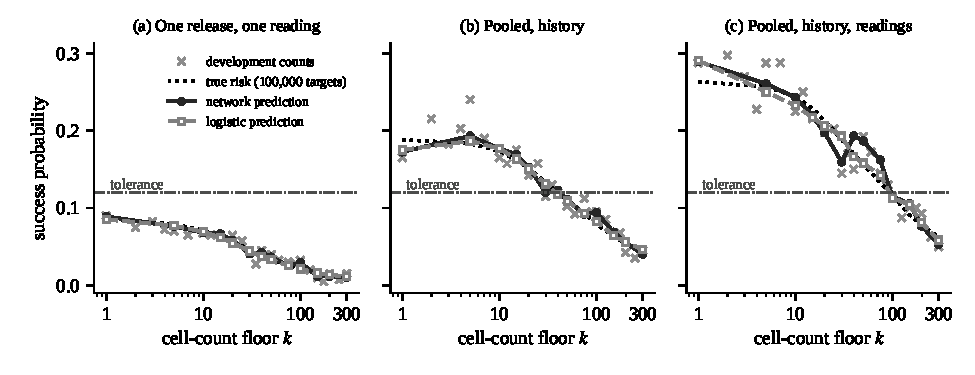
\includegraphics[width=\linewidth]{figures/fig_neural_predictions.pdf}
\caption{What the neural network predicted. For each declared attack, the frozen
predictions of the network (solid line, filled circles) and of the logistic model
(dashed line, open squares) against the true risk estimated from 100{,}000
separate targets (dotted line), with the development success rates the models were
fitted to (crosses, 400 targets each) and the tolerance (dash-dot line). The
network was fitted to the crosses alone and never saw the final audit.}
\label{fig:neural-predictions}
\end{figure}

\begin{table}[t]
\centering
\caption{What the two models learned from the development attacks. Log losses are the binomial log loss per development attack on the training and held-out floors; the epoch is where held-out loss was lowest. Errors compare each model's frozen prediction with the true risk, estimated from 100{,}000 separate targets, over the 39 coordinates of the release grid. The predicted floor is the last floor, from $k=300$ down, at which every predicted risk lies below the tolerance; the start floor is one step stricter.}
\label{tab:neural-fit}
\small\setlength{\tabcolsep}{4pt}
\begin{tabular}{lrrrrrrr}
\toprule
 & \multicolumn{2}{c}{Log loss} & & \multicolumn{2}{c}{Error against truth} & \multicolumn{2}{c}{Floor}\\
\cmidrule(lr){2-3}\cmidrule(lr){5-6}\cmidrule(lr){7-8}
Model & Training & Held out & Epoch & Mean & Largest & Predicted & Start \\
\midrule
Network, two hidden layers & 0.3240 & 0.3482 & 1146 & 0.008 & 0.031 & 100 & 150 \\
Logistic model & 0.3245 & 0.3480 & 2067 & 0.004 & 0.027 & 100 & 150 \\
\bottomrule
\end{tabular}
\end{table}


\subsection{What produces the pooled excess}\label{sec:carried}
In a synthetic population of 200,000 units with a five per cent release sample, four releases that are each 3-anonymous, joined through a persistent pseudonym, have single-release identification probabilities summing to 0.2530, which bounds the chance that some single release succeeds by~\eqref{eq:union}; the pooled attack succeeds with probability 0.4581. On four 3-anonymous variants of a public Census sample of 29,501 records, joined the same way, the corresponding figures are 0.381 and 0.709. These figures are carried over from \cite{mahomane2026}; the credit-register results below are new.

\begin{table}[t]\centering\small
\caption{Share of 4,000 targets named correctly on the synthetic credit register, with the exact one-sided 95 per cent upper bound in brackets. The middle columns change one factor at a time on the same targets; every pooled column assumes the adversary knows the target's history.}\label{tab:carried}
\begin{tabular}{lrcccc}
\toprule
 & & \multicolumn{2}{c}{One release} & \multicolumn{2}{c}{All six releases}\\\cmidrule(lr){3-4}\cmidrule(lr){5-6}
Policy & Kept & One reading & Six readings & One reading & Six readings\\\midrule
No suppression & 27{,}167 & 0.089 (0.097) & 0.158 (0.168) & 0.191 (0.201) & 0.260 (0.272)\\
$k=5$ & 26{,}885 & 0.074 (0.081) & 0.141 (0.150) & 0.183 (0.194) & 0.269 (0.281)\\
$k=10$ & 26{,}019 & 0.070 (0.076) & 0.130 (0.139) & 0.179 (0.190) & 0.244 (0.256)\\\bottomrule
\end{tabular}
\end{table}

Table~\ref{tab:carried} splits the pooled excess. With no suppression, one release and one reading give 0.089 and the full pooled attack 0.260. Six readings in one release give 0.158, and pooling with one reading gives 0.191: the target's history is worth more than five further readings. Pooling works through the history: a candidate whose pattern of appearances differs from the target's is excluded, and the 19 per cent of loans that are not live in every vintage are nearly always found.

\begingroup\let\small\footnotesize\begin{table}[t]
\centering
\caption{What sets the programme floor on the synthetic credit register, tolerance 0.12. History: the adversary knows in which vintages the target's loan is live. The floor is chosen by fixed-sequence testing from $k=300$ down on one draw of 4{,}000 targets and confirmed on a second, independent draw (rate, with exact 95 per cent upper bound); where confirmation fails the next stricter level that passes is shown. Loans and exposure are the percentages of the first release kept at that floor. The subgroup floor requires every size class to meet the tolerance, with the largest firms on a stratified draw, from $k=200$ down. The insider reads exposure with error 0.01 on the log scale. In the Floor column ``none'' means no level up to 300 passes, and in the Subgroup column no level up to 200.}
\label{tab:robust}
\small\setlength{\tabcolsep}{3pt}
\begin{tabular}{lrrrrr}
\toprule
Adversary & Floor & Confirmation & Loans (\%) & Exposure (\%) & Subgroup \\
\midrule
One release, one reading & 1 & 0.084 (0.092) & 100 & 100 & 20 \\
Six releases, one reading, no history & 1 & 0.083 (0.091) & 100 & 100 & -- \\
Six releases, one reading, history & 75 & 0.096 (0.104) & 45 & 11 & 200 \\
Six releases, reading per vintage, no history & 20 & 0.105 (0.114) & 85 & 52 & -- \\
Six releases, reading per vintage, history & 150 & 0.101 (0.109) & 20 & 4 & none \\
Insider: exact exposure, history & none & -- & -- & -- & -- \\
\midrule
\multicolumn{6}{l}{\emph{Exposure published to one significant figure}}\\
One release, one reading & 1 & 0.079 (0.086) & 100 & 100 & -- \\
Six releases, one reading, history & 50 & 0.111 (0.119) & 58 & 20 & -- \\
Six releases, reading per vintage, history & 150 & 0.085 (0.092) & 20 & 4 & -- \\
Insider: exact exposure, history & none & -- & -- & -- & -- \\
\bottomrule
\end{tabular}
\end{table}
\endgroup

Table~\ref{tab:robust} (\nolinkurl{scripts/programme_robustness.py}) chooses the floor for each piece of the adversary's knowledge by fixed-sequence testing from $k=300$ down on one draw of 4{,}000 targets and confirms it on a second. Per release the floor is 1. Six vintages and one reading without the history also give 1; that is a property of the generator, in which published values never change. With the history the selection draw passed $k=50$, but the confirmation draw did not (upper bound 0.123), so the floor is the next stricter level, 75. With a reading per live vintage as well it is 150. Requiring every size class to meet the tolerance gives 20 for a single release and 200 for pooling with the history, and no level up to 200 passes for the full attack. An insider who knows exposure to within one per cent and knows the history defeats every floor up to 300, where it still names 42 per cent of targets. Publishing exposure to one significant figure hardly moves the outsiders' floors, since their readings are noisier than the rounding, but it halves the insider's success (0.388 against 0.772 with no suppression) and cuts the share of loans that published fields alone can relink across vintages from 1.00 to 0.10, which is what would make rotating pseudonyms worth doing. The floors keep little of the file: 75 keeps 45 per cent of loans and 11 per cent of exposure, and 150 keeps 20 and 4 per cent, with no large-firm loans. Table~\ref{tab:tolerance-floors} repeats the selection at tolerances of 0.05, 0.09 and 0.20, from the same draw. It reports the selection floor before confirmation, which is why pooling with the history shows 50 at 0.12 rather than the confirmed 75. The floors move by an order of magnitude across this range: at 0.05 a single release already needs 40 and the full attack has no floor up to 300, while at 0.20 the three outside attacks need 1, 5 and 30. Over 20 independent register draws at the declared reading noise the floors were 1, 40 to 75, and 100 to 150 (Supplement, Section~\ref{S-sec:s-methods}).

\begin{table}[t]
\centering
\caption{The floor chosen at four tolerances by the selection draw of Table~\ref{tab:robust}, before confirmation; at 0.12 pooling with the history therefore shows 50, where Table~\ref{tab:robust} shows the confirmed 75. ``None'' means no level up to 300 passes.}
\label{tab:tolerance-floors}
\small
\begin{tabular}{lrrrr}
\toprule
Tolerance & One release & Pooling, history & Full pooled & Insider \\
\midrule
0.05 & 40 & 300 & none & none \\
0.09 & 5 & 100 & 200 & none \\
0.12 & 1 & 50 & 150 & none \\
0.20 & 1 & 5 & 30 & none \\
\bottomrule
\end{tabular}
\end{table}



\section{What the gate adds to the security of a release process}\label{sec:security}
Disclosure review is a security assessment, and it faces two adversaries. The first, $\mathcal A_{\rm data}$, holds the releases and the declared auxiliary information and tries to identify a unit; the coordinates describe what it can do. The second, $\mathcal A_{\rm op}$, is whoever runs the audit and wants a release to pass, through carelessness, deadline pressure or intent. Per-release review has no model of either. The gate gives a claim about the first that holds only if the second is contained, so we state both.

\paragraph{Security claim.} Let a programme have error budget $\alpha$ and a registry through which every coordinate is registered, every bet is committed and every attack on the confidential register is run. The operator may register coordinates, choose predictable bets and stop audits at will. It wins if the registry calls a release eligible while some attack declared for it succeeds at or above its tolerance. Under Assumption~\ref{ass:law}, Theorem~\ref{thm:gate} and Propositions~\ref{prop:chain} and~\ref{prop:release} bound the operator's chance of winning by $\alpha$, whatever its strategy, provided the following are trusted: (T1) the registry's storage and budget ledger, one per programme and kept across re-assessments; (T2) the randomness from which targets are drawn, which the operator cannot predict when it registers a coordinate; (T3) the attack code, fixed by a digest at registration; (T4) the list of coordinates declared for each release, fixed before its first outcome; and (T5) a time source the operator does not control. The $\sigma$-fields $\F_g$ of Section~\ref{sec:gate} must include everything the operator knows, including any seed; an operator who chooses the seed knows every outcome in advance, and Assumption~\ref{ass:law} fails.

\paragraph{What breaking the trusted parts costs.} Table~\ref{tab:audit-process} measures three ways the operator can break them, on Bernoulli attack streams at a stated risk, with one coordinate at the full level and the bet of Section~\ref{sec:credit}. An operator who can pick among seeds, or who runs shadow audits outside the registry and registers only the one that passed, turns a false-certification rate of 0.038 at the tolerance into 0.32 with ten tries and 0.98 with a hundred; the rates for several tries are computed from the measured single-try rate, treating the tries as independent. An operator who chooses each bet after seeing the outcome certifies an attack that succeeds 20 per cent of the time in every one of 2{,}000 runs of at most 300 draws. The repository implements the matching controls: targets derived from a committed secret and a later round of a public randomness beacon, so that neither the operator nor the beacon alone chooses them; a two-phase coordinate that records each bet in the ledger before the registry runs the attack and records its outcome; and a hash-chained ledger whose entries cannot be changed, dropped or reordered without breaking the chain or changing its head. With them in place, and with the registry trusted, the rates return to the honest ones.

\begin{table}[t]\centering\small
\caption{Attacks on the audit process. Share of runs in which an unsafe or boundary coordinate is certified, with one coordinate at the full level $\alpha=0.05$ and tolerance 0.12. Seed grinding rows use at most 3{,}000 draws and the capped plug-in bet; post-hoc rows use at most 300 draws and the operator's bet without the control, and the capped plug-in bet with it. Tries is the number of seeds or shadow audits the operator can choose among. Without the control, the rate for several tries is $1-(1-f)^{\rm tries}$ for the single-try rate $f$; with it, the operator has one stream. Script: \nolinkurl{scripts/audit_process_attacks.py}.}\label{tab:audit-process}
\begin{tabular}{lrrrr}
\toprule
Attack on the audit & True risk & Tries & Without control & With control\\\midrule
Seed grinding or shadow audits & 0.12 & 1 & 0.038 & 0.038 \\
Seed grinding or shadow audits & 0.12 & 10 & 0.322 & 0.038 \\
Seed grinding or shadow audits & 0.12 & 100 & 0.979 & 0.038 \\
Seed grinding or shadow audits & 0.14 & 1 & 0.007 & 0.007 \\
Seed grinding or shadow audits & 0.14 & 10 & 0.066 & 0.007 \\
Seed grinding or shadow audits & 0.14 & 100 & 0.495 & 0.007 \\
Bet chosen after the outcome & 0.14 & 1 & 1.000 & 0.007 \\
Bet chosen after the outcome & 0.20 & 1 & 1.000 & 0.000 \\
\bottomrule
\end{tabular}
\end{table}


\paragraph{What the gate adds.} Against $\mathcal A_{\rm data}$, over per-release review, it adds programme coverage (pooled attacks are coordinates of their own, and Proposition~\ref{prop:pool} shows no per-release figure stands in for them), error-controlled assurance (each certificate carries its error share, protocol and number of draws), fail-closed defaults (an unaudited attack is not zero risk, and a chain stops at its first failure) and a place for red-team findings (a new attack can be registered at any time without voiding certificates already issued, if budget was reserved for it). Against $\mathcal A_{\rm op}$ it makes audit shopping either impossible or paid for out of the budget, but only under complete mediation \cite{saltzer1975}: every attack run on the confidential register must pass through the registry, and development work must use a separate extract.

\paragraph{What it does not add.} The implementation is a library, not a security boundary. Python cannot stop code in the same process from changing private state, and the hash chain detects changes only if its head is published or time-stamped outside the operator's control. A deployment that must hold against the operator needs the registry as a separate service with its own storage, signing keys and time stamps, separation of duties (an independent team writes and signs the attack code; a data custodian holds the register and the randomness commitment; the owner signs the tolerance before the first outcome), and verification by internal audit inside the secure environment, since the log of which targets were identified is itself confidential. The certificate covers the declared attack protocols only. It is not differential privacy and gives no guarantee against an adversary outside the declared set. In the terms of security practice, the coordinate list is the output of threat modelling \cite{shostack2014}, the audits are red-team tests with a sampling design, and the decision record is an assurance case; we claim no conformity with any standard, and a deployment should be reviewed against de-identification guidance such as \cite{nist800188}.

\section{Discussion and limitations}\label{sec:discussion}
\paragraph{What is certified.} A certificate covers the declared coordinates only. It says nothing about attacks that were not registered, and registering a convenient subset and calling it the programme is a failure of governance that no bound corrects. The gate controls the probability of certifying an unsafe coordinate; it does not supply a risk estimate. Where a numerical figure is needed, an audited margin $z_i=1-\overline{R}_i/\tau_i$ must be computed from a valid upper bound $\overline{R}_i$ (Section~\ref{sec:decision}), not from $E_{i,b}$.

\paragraph{When Assumption~\ref{ass:law} fails.} The sampling condition fails under reused targets, hidden target features shared between interleaved streams, or changes to the attacker after outcomes are seen. The supplement gives a two-line example in which reusing a failed target lets evidence grow without bound. Where a deviation $\kappa_i$ from the condition can be justified from outside the audit, the betting denominator can be lowered to $\tau_i-\kappa_i$ with bets restricted to $[0,\tau_i-\kappa_i)$, at a cost in power (Supplement, Section~\ref{S-sec:s-filtration}). The credit experiment draws fresh targets for every coordinate; we did not run a case in which targets are reused.

\paragraph{The pooled threat model.} On the register studied, the programme effect needs the adversary to know the target loan's history. Without it pooling adds nothing, but that is a property of the generator, in which a loan's published key and exposure never change; on a real register, where outstanding amounts move every month, the other vintages would carry information through the path of exposures. With the history the floor rises from 1 to 75, and with a reading per vintage as well to 150. Who holds the history matters: the borrower, its lenders and parties to a registered charge know it, and most of them also know the exposure exactly, which is the insider row of Table~\ref{tab:robust}; a journalist working from the releases usually does not. Which adversary to declare is the agency's decision, and the answer moves the floor more than any choice of audit design. It must be declared before the audit.

\paragraph{What needs e-processes.} Registering coordinates after reading results does not by itself need e-processes: online alpha-spending over fixed-sample tests on fresh targets is also valid under Assumption~\ref{ass:law}. The gate is needed when an audit may be stopped, extended or read before its planned size. Its practical value is that monitoring is free, so an audit can stop as soon as the evidence is clear and can continue when a reviewer asks for more without voiding what has been done.

\paragraph{Cost of adaptivity.} The release chain used a median of 6{,}422 attacks, against 9{,}002 for the same gate with every coordinate registered at the start and stopped at the first failure, 13{,}764 for one chain per attack at $\alpha/3$, and 10{,}000 to 36{,}000 for the fixed designs. The fixed-sequence test with 3{,}000 attacks per coordinate found the estimated true floor of 100 in 4 streams against the release chain's 1, because at $k=100$ the full attack succeeds at 0.116, above the cap on the bet and so close to the tolerance that the capped bet certifies it only by chance, and even the best fixed bet would need about 43{,}000 draws on average (Proposition~\ref{prop:length}). Where the grid and budget are known in advance and the audit will not be read before it ends, a fixed-sample design does as well; the gate is worth its cost when audits stop early or are read as they run.

\paragraph{Shift in the attack law.} The gate certifies the declared attack under the registered target law. If an agency can justify, from outside the audit, that the law an attacker will face differs from the audited one by at most $\rho$ in total variation, a fixed-family audit gives a bound of the audited upper bound plus $\rho$ for every coordinate at once; the supplement (Section~\ref{S-sec:multiscale-extension}) states it with its zero-success sample size, together with the mathematics of a multiscale proposal model. Neither is used in the results, and a change of attack algorithm is not a shift of this kind.

\paragraph{Other failure modes.} A zero-alternative bet ends on its first success, and a bet capped well below the true risk wastes power. Error allocated to a finished coordinate cannot be reclaimed, and a reserve for later coordinates must be recorded before it is spent. A programme that would accept a share of false certifications in return for power could control a false discovery rate instead \cite{benjamini1995,javanmard2018,wang2022}; we have not studied that choice.

\paragraph{What the code does.} The gate implementation certifies at first crossing and then refuses further outcomes. Its public fields are read-only, which guards against programming mistakes but not against code that changes private state. Chains and release chains open the next setting only after the current one passes. The two-phase coordinate records each bet before the attack runs, and the ledger is hash-chained; the underlying coordinate still accepts outcomes from any caller, so the two-phase path binds only when the registry enforces it. The eligibility check covers only the coordinates the caller names; no code can check that the declared coordinate set is complete or that attack draws satisfy Assumption~\ref{ass:law}.

\paragraph{Separate search evaluation.} A further public-file experiment in Supplement Section~\ref{S-sec:public-search} compares random, informed heuristic, Sobol and neural-guided scenario search over 30 Census state samples, with matched development and fresh-confirmation budgets. Neural targeting confirms many high-risk settings but covers fewer distinct scenario cells than Sobol. A fifth arm, a 4.0B-parameter open-weight language model run locally under the same prompt and budget, covers fewer cells still (6.05 against 13.65 over the 20 states for which it returned a valid list): it copied the front of the catalogue rather than searching it. This is conditional empirical-file evidence for one declared attack; it neither changes the synthetic-register gate results nor establishes an LLM advantage.

\section{Conclusion}\label{sec:conclusion}
A release programme needs a certificate for every attack it declares, including pooled attacks on several vintages, and the list of attacks will grow as audits are read. Online alpha-spending over betting test supermartingales gives such a certificate with familywise control, provided attack targets are sampled so that Assumption~\ref{ass:law} holds and the operator cannot choose them. Its cost is set by the gap between risk and tolerance, and release chains let an agency search an ordered grid of settings against several declared attacks without splitting its budget. On a synthetic credit register the floor depends on what the adversary is assumed to know, above all the target's history and the precision of its exposure readings, and against an adversary who knows the history the floors that meet the tolerance leave little of the file. For such an adversary a loan-level release is the wrong product, and aggregate tables or access in a secure setting are the realistic choices. Testing the gate on a real register remains to be done.

\section*{Data and code availability}
The companion repository, \url{https://github.com/Nube1/privacy-risk-thresholds} (version 0.7.0), contains the synthetic register, the public-file adapters, the gate implementation, its tests and the scripts that produce every table: \nolinkurl{scripts/adaptive_audit_comparison.py} for Table~\ref{tab:new-audit}, \nolinkurl{scripts/adaptive_audit_chain.py} for Table~\ref{tab:chain-audit}, \nolinkurl{scripts/programme_robustness.py} for the floors in Section~\ref{sec:carried}, \nolinkurl{scripts/audit_process_attacks.py} for Table~\ref{tab:audit-process}, \nolinkurl{privacy_risk.neural_pipeline} for Table~\ref{tab:neural-pipeline}, and the pipeline of \cite{mahomane2026} for Table~\ref{tab:carried}. No confidential register is supplied. The supplement lists the commands.

\begin{thebibliography}{99}\small
\bibitem{abowd2018} Abowd, J. M. (2018). The U.S. Census Bureau adopts differential privacy. In \emph{Proceedings of the 24th ACM SIGKDD International Conference on Knowledge Discovery and Data Mining}, 2867.
\bibitem{aharoni2014} Aharoni, E. and Rosset, S. (2014). Generalized $\alpha$-investing: definitions, optimality results and application to public databases. \emph{Journal of the Royal Statistical Society, Series B} 76(4), 771--794.
\bibitem{bates2021} Bates, S., Angelopoulos, A., Lei, L., Malik, J. and Jordan, M. I. (2021). Distribution-free, risk-controlling prediction sets. \emph{Journal of the ACM} 68(6), 1--34.
\bibitem{benjamini1995} Benjamini, Y. and Hochberg, Y. (1995). Controlling the false discovery rate: a practical and powerful approach to multiple testing. \emph{Journal of the Royal Statistical Society, Series B} 57(1), 289--300.
\bibitem{berk2013} Berk, R., Brown, L., Buja, A., Zhang, K. and Zhao, L. (2013). Valid post-selection inference. \emph{Annals of Statistics} 41(2). doi:10.1214/12-AOS1077.
\bibitem{carlini2022} Carlini, N., Chien, S., Nasr, M., Song, S., Terzis, A. and Tram\`er, F. (2022). Membership inference attacks from first principles. In \emph{2022 IEEE Symposium on Security and Privacy}, 1897--1914.
\bibitem{clopper1934} Clopper, C. J. and Pearson, E. S. (1934). The use of confidence or fiducial limits illustrated in the case of the binomial. \emph{Biometrika} 26(4), 404--413.
\bibitem{cohen2020} Cohen, A. and Nissim, K. (2020). Towards formalizing the GDPR's notion of singling out. \emph{Proceedings of the National Academy of Sciences} 117(15), 8344--8352.
\bibitem{darling1967} Darling, D. A. and Robbins, H. (1967). Confidence sequences for mean, variance, and median. \emph{Proceedings of the National Academy of Sciences} 58(1), 66--68.
\bibitem{dinur2003} Dinur, I. and Nissim, K. (2003). Revealing information while preserving privacy. In \emph{Proceedings of the 22nd ACM Symposium on Principles of Database Systems}, 202--210.
\bibitem{dong2022} Dong, J., Roth, A. and Su, W. J. (2022). Gaussian differential privacy. \emph{Journal of the Royal Statistical Society, Series B} 84(1), 3--37.
\bibitem{duncan1989} Duncan, G. T. and Lambert, D. (1989). The risk of disclosure for microdata. \emph{Journal of Business and Economic Statistics} 7(2), 207--217.
\bibitem{dunn1961} Dunn, O. J. (1961). Multiple comparisons among means. \emph{Journal of the American Statistical Association} 56(293), 52--64.
\bibitem{dwork2014} Dwork, C. and Roth, A. (2014). The algorithmic foundations of differential privacy. \emph{Foundations and Trends in Theoretical Computer Science} 9(3--4), 211--407.
\bibitem{elemam2008} El Emam, K. and Dankar, F. K. (2008). Protecting privacy using $k$-anonymity. \emph{Journal of the American Medical Informatics Association} 15(5), 627--637.
\bibitem{elemam2011} El Emam, K., Jonker, E., Arbuckle, L. and Malin, B. (2011). A systematic review of re-identification attacks on health data. \emph{PLoS ONE} 6(12), e28071.
\bibitem{foster2008} Foster, D. P. and Stine, R. A. (2008). $\alpha$-investing: a procedure for sequential control of expected false discoveries. \emph{Journal of the Royal Statistical Society, Series B} 70(2), 429--444.
\bibitem{ganta2008} Ganta, S. R., Kasiviswanathan, S. P. and Smith, A. (2008). Composition attacks and auxiliary information in data privacy. In \emph{Proceedings of the 14th ACM SIGKDD International Conference on Knowledge Discovery and Data Mining}, 265--273.
\bibitem{grunwald2024} Gr\"unwald, P., de Heide, R. and Koolen, W. (2024). Safe testing. \emph{Journal of the Royal Statistical Society, Series B} 86(5), 1091--1128.
\bibitem{howard2020} Howard, S. R., Ramdas, A., McAuliffe, J. and Sekhon, J. (2020). Time-uniform Chernoff bounds via nonnegative supermartingales. \emph{Probability Surveys} 17. doi:10.1214/18-PS321.
\bibitem{howard2021} Howard, S. R., Ramdas, A., McAuliffe, J. and Sekhon, J. (2021). Time-uniform, nonparametric, nonasymptotic confidence sequences. \emph{Annals of Statistics} 49(2), 1055--1080.
\bibitem{hundepool2012} Hundepool, A., Domingo-Ferrer, J., Franconi, L., Giessing, S., Schulte Nordholt, E., Spicer, K. and de Wolf, P.-P. (2012). \emph{Statistical Disclosure Control}. Wiley.
\bibitem{jagielski2020} Jagielski, M., Ullman, J. and Oprea, A. (2020). Auditing differentially private machine learning: how private is private SGD? In \emph{Advances in Neural Information Processing Systems} 33, 22205--22216.
\bibitem{javanmard2018} Javanmard, A. and Montanari, A. (2018). Online rules for control of false discovery rate and false discovery exceedance. \emph{Annals of Statistics} 46(2). doi:10.1214/17-AOS1559.
\bibitem{johari2022} Johari, R., Koomen, P., Pekelis, L. and Walsh, D. (2022). Always valid inference: continuous monitoring of A/B tests. \emph{Operations Research} 70(3), 1806--1821.
\bibitem{kairouz2017} Kairouz, P., Oh, S. and Viswanath, P. (2017). The composition theorem for differential privacy. \emph{IEEE Transactions on Information Theory} 63(6), 4037--4049.
\bibitem{kasiviswanathan2014} Kasiviswanathan, S. P. and Smith, A. (2014). On the `semantics' of differential privacy: a Bayesian formulation. \emph{Journal of Privacy and Confidentiality} 6(1).
\bibitem{khwaja2008} Khwaja, A. I. and Mian, A. (2008). Tracing the impact of bank liquidity shocks: evidence from an emerging market. \emph{American Economic Review} 98(4), 1413--1442.
\bibitem{kifer2011} Kifer, D. and Machanavajjhala, A. (2011). No free lunch in data privacy. In \emph{Proceedings of the 2011 ACM SIGMOD International Conference on Management of Data}, 193--204.
\bibitem{kifer2014} Kifer, D. and Machanavajjhala, A. (2014). Pufferfish: a framework for mathematical privacy definitions. \emph{ACM Transactions on Database Systems} 39(1), 1--36.
\bibitem{lai1976} Lai, T. L. (1976). On confidence sequences. \emph{Annals of Statistics} 4(2). doi:10.1214/aos/1176343406.
\bibitem{mahomane2026} Mahomane, R. R. M. (2026). Governing privacy risk across repeated statistical releases: probability models, programme tolerances and accountable decisions. Author manuscript, supplied to the editor with this submission; an earlier version was presented at the Banco de Portugal and IFC Workshop on Data Security and Privacy, Lisbon, September 2026. The companion repository reproduces every result in it.
\bibitem{demontjoye2013} de Montjoye, Y.-A., Hidalgo, C. A., Verleysen, M. and Blondel, V. D. (2013). Unique in the crowd: the privacy bounds of human mobility. \emph{Scientific Reports} 3, 1376.
\bibitem{narayanan2008} Narayanan, A. and Shmatikov, V. (2008). Robust de-anonymization of large sparse datasets. In \emph{2008 IEEE Symposium on Security and Privacy}, 111--125.
\bibitem{nasr2021} Nasr, M., Song, S., Thakurta, A., Papernot, N. and Carlini, N. (2021). Adversary instantiation: lower bounds for differentially private machine learning. In \emph{2021 IEEE Symposium on Security and Privacy}, 866--882.
\bibitem{ramdas2023} Ramdas, A., Gr\"unwald, P., Vovk, V. and Shafer, G. (2023). Game-theoretic statistics and safe anytime-valid inference. \emph{Statistical Science} 38(4), 576--601.
\bibitem{reiter2005} Reiter, J. P. (2005). Estimating risks of identification disclosure in microdata. \emph{Journal of the American Statistical Association} 100(472), 1103--1112.
\bibitem{robbins1970} Robbins, H. (1970). Statistical methods related to the law of the iterated logarithm. \emph{Annals of Mathematical Statistics} 41(5), 1397--1409.
\bibitem{rocher2019} Rocher, L., Hendrickx, J. M. and de Montjoye, Y.-A. (2019). Estimating the success of re-identifications in incomplete datasets using generative models. \emph{Nature Communications} 10, 3069.
\bibitem{shafer2019} Shafer, G. and Vovk, V. (2019). \emph{Game-Theoretic Foundations for Probability and Finance}. Wiley, Hoboken.
\bibitem{shafer2011} Shafer, G., Shen, A., Vereshchagin, N. and Vovk, V. (2011). Test martingales, Bayes factors and $p$-values. \emph{Statistical Science} 26(1), 84--101.
\bibitem{shlomo2010} Shlomo, N. and Skinner, C. (2010). Assessing the protection provided by misclassification-based disclosure limitation methods for survey microdata. \emph{Annals of Applied Statistics} 4(3). doi:10.1214/09-AOAS317.
\bibitem{shokri2017} Shokri, R., Stronati, M., Song, C. and Shmatikov, V. (2017). Membership inference attacks against machine learning models. In \emph{2017 IEEE Symposium on Security and Privacy}, 3--18.
\bibitem{skinner2008} Skinner, C. J. and Shlomo, N. (2008). Assessing identification risk in survey microdata using log-linear models. \emph{Journal of the American Statistical Association} 103(483), 989--1001.
\bibitem{steinke2023} Steinke, T., Nasr, M. and Jagielski, M. (2023). Privacy auditing with one (1) training run. In \emph{Advances in Neural Information Processing Systems} 36, 49268--49280.
\bibitem{sweeney2002} Sweeney, L. (2002). $k$-anonymity: a model for protecting privacy. \emph{International Journal of Uncertainty, Fuzziness and Knowledge-Based Systems} 10(5), 557--570.
\bibitem{tian2021} Tian, J. and Ramdas, A. (2021). Online control of the familywise error rate. \emph{Statistical Methods in Medical Research} 30(4), 976--993.
\bibitem{ville1939} Ville, J. (1939). \emph{\'Etude critique de la notion de collectif}. Gauthier-Villars, Paris.
\bibitem{vovk2021} Vovk, V. and Wang, R. (2021). E-values: calibration, combination and applications. \emph{Annals of Statistics} 49(3). doi:10.1214/20-AOS2020.
\bibitem{wald1945} Wald, A. (1945). Sequential tests of statistical hypotheses. \emph{Annals of Mathematical Statistics} 16(2), 117--186.
\bibitem{wang2006} Wang, K. and Fung, B. C. M. (2006). Anonymizing sequential releases. In \emph{Proceedings of the 12th ACM SIGKDD International Conference on Knowledge Discovery and Data Mining}, 414--423.
\bibitem{wang2022} Wang, R. and Ramdas, A. (2022). False discovery rate control with e-values. \emph{Journal of the Royal Statistical Society, Series B} 84(3), 822--852.
\bibitem{wasserman2010} Wasserman, L. and Zhou, S. (2010). A statistical framework for differential privacy. \emph{Journal of the American Statistical Association} 105(489), 375--389.
\bibitem{waudby2024} Waudby-Smith, I. and Ramdas, A. (2024). Estimating means of bounded random variables by betting. \emph{Journal of the Royal Statistical Society, Series B} 86(1), 1--27.
\bibitem{xu2024} Xu, Z., Karampatziakis, N. and Mineiro, P. (2024). Active, anytime-valid risk controlling prediction sets. In \emph{Advances in Neural Information Processing Systems} 37.
\bibitem{zhou2026} Zhou, S., Vossler, P., Sivaraman, V., Mai, Y. and Feng, J. (2026). Adaptive auditing of AI systems with anytime-valid guarantees. arXiv:2605.07002.
\bibitem{maurer1995} Maurer, W., Hothorn, L. A. and Lehmacher, W. (1995). Multiple comparisons in drug clinical trials and preclinical assays: a-priori ordered hypotheses. In J. Vollmar (ed.), \emph{Biometrie in der chemisch-pharmazeutischen Industrie} 6, 3--18. Fischer, Stuttgart.
\bibitem{stark2008} Stark, P. B. (2008). Conservative statistical post-election audits. \emph{Annals of Applied Statistics} 2(2), 550--581.
\bibitem{stark2023} Stark, P. B. (2023). ALPHA: audit that learns from previously hand-audited ballots. \emph{Annals of Applied Statistics} 17(1), 641--679.
\bibitem{wald1944} Wald, A. (1944). On cumulative sums of random variables. \emph{Annals of Mathematical Statistics} 15(3), 283--296.
\bibitem{waudby2021} Waudby-Smith, I., Stark, P. B. and Ramdas, A. (2021). RiLACS: risk-limiting audits via confidence sequences. In \emph{Electronic Voting (E-Vote-ID 2021)}, Lecture Notes in Computer Science 12900, 124--139.
\bibitem{xiao2007} Xiao, X. and Tao, Y. (2007). $m$-invariance: towards privacy preserving re-publication of dynamic datasets. In \emph{Proceedings of the 2007 ACM SIGMOD International Conference on Management of Data}, 689--700.
\bibitem{berger1982} Berger, R. L. (1982). Multiple parameter hypothesis testing and acceptance sampling. \emph{Technometrics} 24(4), 295--300.
\bibitem{bretz2009} Bretz, F., Maurer, W., Brannath, W. and Posch, M. (2009). A graphical approach to sequentially rejective multiple test procedures. \emph{Statistics in Medicine} 28(4), 586--604.
\bibitem{dmitrienko2007} Dmitrienko, A. and Tamhane, A. C. (2007). Gatekeeping procedures with clinical trial applications. \emph{Pharmaceutical Statistics} 6(3), 171--180.
\bibitem{hsu1999} Hsu, J. C. and Berger, R. L. (1999). Stepwise confidence intervals without multiplicity adjustment for dose-response and toxicity studies. \emph{Journal of the American Statistical Association} 94(446), 468--482.
\bibitem{kaufmann2016} Kaufmann, E., Capp\'e, O. and Garivier, A. (2016). On the complexity of best-arm identification in multi-armed bandit models. \emph{Journal of Machine Learning Research} 17(1), 1--42.
\bibitem{krichevsky1981} Krichevsky, R. and Trofimov, V. (1981). The performance of universal encoding. \emph{IEEE Transactions on Information Theory} 27(2), 199--207.
\bibitem{nist800188} Garfinkel, S., Near, J., Dajani, A., Singer, P. and Guttman, B. (2023). \emph{De-Identifying Government Datasets: Techniques and Governance}. NIST Special Publication 800-188. National Institute of Standards and Technology.
\bibitem{saltzer1975} Saltzer, J. H. and Schroeder, M. D. (1975). The protection of information in computer systems. \emph{Proceedings of the IEEE} 63(9), 1278--1308.
\bibitem{shostack2014} Shostack, A. (2014). \emph{Threat Modeling: Designing for Security}. Wiley, Indianapolis.
\bibitem{gdpr2016} European Parliament and Council (2016). Regulation (EU) 2016/679 (General Data Protection Regulation), Article 4(5) and Recital 26. \emph{Official Journal of the European Union} L 119, 1--88.
\bibitem{bichsel2021} Bichsel, B., Steffen, S., Bogunovic, I. and Vechev, M. (2021). DP-Sniper: black-box discovery of differential privacy violations using classifiers. In \emph{2021 IEEE Symposium on Security and Privacy}, 391--409.
\bibitem{chugg2023} Chugg, B., Cortes-Gomez, S., Wilder, B. and Ramdas, A. (2023). Auditing fairness by betting. In \emph{Advances in Neural Information Processing Systems} 36.
\bibitem{ding2018} Ding, Z., Wang, Y., Wang, G., Zhang, D. and Kifer, D. (2018). Detecting violations of differential privacy. In \emph{Proceedings of the 2018 ACM SIGSAC Conference on Computer and Communications Security}, 475--489.
\bibitem{nasr2023} Nasr, M., Hayes, J., Steinke, T., Balle, B., Tram\`er, F., Jagielski, M., Carlini, N. and Terzis, A. (2023). Tight auditing of differentially private machine learning. In \emph{32nd USENIX Security Symposium}, 1631--1648.
\bibitem{stadler2022} Stadler, T., Oprisanu, B. and Troncoso, C. (2022). Synthetic data: anonymisation groundhog day. In \emph{31st USENIX Security Symposium}, 1451--1468.
\bibitem{ec2533} Council of the European Union (1998). Council Regulation (EC) No 2533/98 concerning the collection of statistical information by the European Central Bank, Article 8, as amended by Council Regulation (EC) No 951/2009. \emph{Official Journal of the European Communities} L 318, 8--19.
\bibitem{ema2016} European Medicines Agency (2016). \emph{External guidance on the implementation of the European Medicines Agency policy on the publication of clinical data for medicinal products for human use}. EMA/90915/2016, London.
\end{thebibliography}
\end{document}
